\documentclass[11pt,a4paper]{article}

\usepackage[french]{babel}
\usepackage[T1]{fontenc}
\usepackage[utf8]{inputenc}
\usepackage{lmodern}
\usepackage[margin=2.4cm]{geometry}
\usepackage{graphicx}
\usepackage{booktabs}
\usepackage{amsmath}
\usepackage{caption}
\usepackage{float}

\title{Projet SDP\\Apprentissage de modèles MR-Sort}
\author{%
Aurélien Delest\\
Robin Capelle\\
Thomas de la Grand'rive\\[0.8em]
Mention IA, 2026--2027}
\date{}

\begin{document}
\maketitle

\begin{abstract}
\noindent
Ce rapport rassemble les résultats des trois jalons. Le jalon~1 apprend un modèle MR-Sort exact par programme linéaire en nombres entiers. Le jalon~2 apprend deux modèles mélangés par une heuristique. Le jalon~3 place cet apprentissage dans un échange entre un émetteur~A et un récepteur~B, brouillé par un agent malveillant. Sur les essais du jalon~1, le modèle appris classe comme le modèle d'origine dans 94~\% des cas. Au jalon~2, deux modèles expliquent 99~\% des objets sans bruit et 91~\% avec 10~\% de bruit, mais les proportions des segments ne sont retrouvées qu'à une dizaine de points près. Au jalon~3, un malveillant qui envoie autant d'objets que~A fait chuter~B. La chute est plus forte si le malveillant met tous ses objets dans la catégorie la plus basse, ou s'il utilise un modèle extrême.
\end{abstract}

\section{Jalon 1 : un modèle MR-Sort}

Un objet est décrit par $n$ notes à maximiser. Il est affecté à une catégorie parmi $p$, de la pire à la meilleure. Pour franchir une frontière, la somme des poids des critères sur lesquels il atteint le profil doit dépasser un seuil de majorité $\lambda$. Les poids sont positifs et de somme~1.

Le modèle est appris par un programme linéaire en nombres entiers, résolu avec Gurobi. L'objectif est de restituer le mieux possible un ensemble d'apprentissage dont les catégories sont connues.

Sur \texttt{dataset0} (60 objets, 5 critères, 3 catégories), Gurobi restitue les 60 objets. Le contrôle par la règle MR-Sort confirme cette restitution.

Le protocole du sujet est ensuite répété 20 fois. Un modèle d'origine est tiré au hasard, 100 objets d'apprentissage sont classés par ce modèle, le programme apprend un modèle, et 10\,000 objets de test comparent les deux. La configuration est celle de \texttt{dataset0} : 5 critères, 3 catégories, notes dans $[0,100]$. Les modèles d'origine qui laissent une catégorie vide sont écartés.

\begin{center}
\begin{tabular}{lc}
\toprule
Qualité moyenne & $0{,}937 \pm 0{,}028$ \\
Qualité minimale & $0{,}878$ \\
Temps moyen de résolution & $0{,}62$~s \\
\bottomrule
\end{tabular}
\end{center}

La qualité est la proportion d'objets de test classés de la même façon par le modèle d'origine et par le modèle appris. L'apprentissage exact retrouve donc le comportement du modèle d'origine, avec un écart d'environ six points.

Le nombre d'objets d'apprentissage fixe la taille du programme. Chaque objet ajoute une variable $\gamma_k$ et, pour chaque frontière qu'il doit respecter, $n$ variables binaires et $5n$ contraintes. Avec 5 critères et 3 catégories, cela fait au plus 1\,100 binaires pour 100 objets et 5\,500 pour 500 objets. Le modèle grossit linéairement, mais le temps de résolution non : la recherche arborescente porte sur ces binaires, et les contraintes de type big-M donnent une relaxation peu serrée.

\begin{center}
\begin{tabular}{lcc}
\toprule
Objets d'apprentissage & 100 & 500 \\
\midrule
Qualité moyenne & $0{,}937$ & $0{,}988$ \\
Temps moyen & $0{,}62$~s & $14{,}6$~s \\
Temps maximal & $1{,}3$~s & $53$~s \\
\bottomrule
\end{tabular}
\end{center}

Passer de 100 à 500 objets gagne cinq points de qualité, mais multiplie le temps moyen par 23. Le pire essai approche la limite de 120~s fixée à Gurobi. Au-delà, l'optimalité ne serait plus garantie. 100 objets suffisent donc à valider la méthode exacte. Ce coût explique aussi le passage à une heuristique au jalon~2, où les fichiers comptent de 300 à 1\,200 objets et jusqu'à 10 critères.

\section{Jalon 2 : deux modèles mélangés}

Les clients d'un supermarché n'ont pas tous le même comportement. Les données mélangent deux segments, et l'appartenance de chaque produit est inconnue. Il faut à la fois retrouver la partition et apprendre un MR-Sort par segment. Le problème est traité par l'heuristique de la bibliothèque lincs, car la version exacte du jalon~1 devient trop coûteuse.

L'algorithme alterne deux étapes, sur le modèle d'un $k$-means. On apprend un modèle par segment, puis chaque objet est envoyé au modèle qui l'explique le mieux. L'explication compare d'abord l'écart de catégorie, puis la marge. Un objet ne change de segment que si l'autre modèle l'explique strictement mieux. Quatre départs sont lancés : un départ guidé par les erreurs d'un modèle unique, et trois départs aléatoires. On retient le départ qui explique le plus d'objets, puis chaque modèle est réappris plus longtemps. L'algorithme ne connaît ni la taille des segments ni le niveau de bruit. Partager les objets compatibles avec les deux modèles a été essayé : cela n'améliorait pas la précision et coûtait environ 23~\% de temps en plus. Cette option a été abandonnée.

L'arrêt a lui aussi été choisi après essais. Une première version s'arrêtait quand la précision d'apprentissage dépassait un seuil fixe, 0,95 puis 0,97. Avec 10~\% de bruit, ce seuil n'était jamais atteint, et la boucle allait jusqu'au nombre maximal d'itérations. L'algorithme s'arrête donc quand la partition ne change plus, ce qui ne suppose rien sur le bruit. Un arrêt sur un jeu de validation a aussi été essayé : il prenait des objets à l'apprentissage sans améliorer la précision de test.

\subsection*{Ce qui est mesuré}

Le jalon~2 demande d'expliquer les données, pas de prédire. On cherche deux MR-Sort qui, à eux deux, rendent compte du plus grand nombre d'objets. La mesure est donc la part des objets d'apprentissage bien classés par au moins un des deux modèles. C'est aussi ce que l'algorithme maximise.

Cette mesure ne vaut pas une précision de prédiction. Pour un objet nouveau, on ne connaît pas sa catégorie, et rien ne dit quel modèle appliquer. Choisir entre deux modèles sans cette information est le problème du jalon~3, où B doit décider lequel des deux modèles appris est celui de A. Au jalon~2, on rend compte de deux choses : la part d'objets expliqués, et les proportions des deux segments, comparées après coup aux valeurs du nom de fichier.

Les résultats portent sur les 36 fichiers de type~A (6 par combinaison de critères, de catégories et de bruit), appris sur 100~\% de leurs objets. Ils sont dans \texttt{results/jalon2\_explication.csv}. Un objet est dit ambigu s'il est bien classé par les deux modèles. La partition aléatoire sert de référence : deux modèles appris chacun sur une moitié tirée au hasard, sans réaffectation.

\begin{center}
\begin{tabular}{llcccc}
\toprule
Bruit & Critères / catégories & 1 modèle & Partition aléatoire & 2 modèles & Ambigus \\
\midrule
Sans bruit & 6 / 3 & 0,792 & 0,878 & 0,993 & 0,46 \\
 & 8 / 4 & 0,776 & 0,877 & 0,994 & 0,36 \\
 & 10 / 5 & 0,795 & 0,863 & 0,980 & 0,35 \\
 & Ensemble & 0,788 & 0,873 & 0,989 & 0,39 \\
\midrule
10~\% & 6 / 3 & 0,717 & 0,812 & 0,924 & 0,19 \\
 & 8 / 4 & 0,669 & 0,810 & 0,919 & 0,26 \\
 & 10 / 5 & 0,704 & 0,778 & 0,895 & 0,25 \\
 & Ensemble & 0,697 & 0,800 & 0,913 & 0,23 \\
\bottomrule
\end{tabular}
\end{center}

Sans bruit, deux modèles expliquent 0,99 des objets, et un seul modèle 0,79. Cet écart a deux causes. Deux modèles ont deux fois plus de paramètres, et chaque objet est compté juste dès que l'un des deux le classe bien : la partition aléatoire, qui ne segmente rien, atteint déjà 0,87. La réaffectation ajoute 12~points de plus. C'est l'apport propre de la segmentation.

Avec 10~\% de bruit, la part expliquée tombe à 0,91, et baisse un peu quand le modèle grossit. Si le bruit change la catégorie de 10~\% des objets, aucun MR-Sort ne les explique, sauf si l'autre modèle leur donne cette catégorie par hasard. On attend donc environ 0,90. Les 0,91 obtenus sont proches de ce plafond : l'algorithme absorbe peu de bruit. L'apport de la segmentation reste de 11~points sur la partition aléatoire.

Entre 19 et 46~\% des objets sont ambigus. Leur segment n'est pas déterminé par les données : ils peuvent passer d'un côté ou de l'autre sans rien changer à la part expliquée.

\begin{center}
\begin{tabular}{lccc}
\toprule
Part du petit segment & Attendue & Trouvée, sans bruit & Trouvée, 10~\% de bruit \\
\midrule
Segments 50/50 (9 + 9 fichiers) & 0,50 & 0,43 & 0,38 \\
Segments 75/25 (9 + 9 fichiers) & 0,25 & 0,31 & 0,33 \\
\bottomrule
\end{tabular}
\end{center}

Les proportions ne sont retrouvées qu'à une dizaine de points près, et le petit segment trouvé reste entre 0,31 et 0,43 quelle que soit la répartition réelle. C'est la conséquence des objets ambigus : avec près d'un tiers des objets attribuables aux deux segments, la proportion n'est fixée qu'à cette marge près. Une part expliquée élevée ne garantit donc pas d'avoir retrouvé les vrais segments.

\section{Jalon 3 : A, B et un agent malveillant}

A envoie à B des objets classés par son modèle MR-Sort. A a peu de calcul : il transmet ce qu'il observe, il n'envoie pas le modèle. Un agent malveillant peut ajouter au plus un objet par objet de A. Il choisit lui-même le vecteur et la catégorie. B reçoit le mélange, sans savoir qui a envoyé quoi, et doit retrouver le modèle de A.

Les essais utilisent 6 critères, 3 catégories et 300 objets de A. Le jeu de test compte 1\,000 objets tirés comme ceux de A et classés par son modèle. La précision est la part de ces objets classés comme A le ferait. Quand B n'apprend que sur les objets de A, cette précision vaut environ 0,98.

\subsection{Malveillant basique}

Le malveillant basique tire un MR-Sort au hasard, avec le même générateur que A, et étiquette ses objets avec ce modèle. B peut répondre de deux façons. Le modèle unique apprend un seul MR-Sort sur tout le mélange. Le choix de B apprend deux modèles, par l'algorithme du jalon~2, puis garde celui qui classe correctement le plus d'objets reçus. Il ne voit pas la source de chaque objet. Si A a envoyé davantage, son modèle recolle à davantage d'objets. Si les deux en envoient autant, les deux comptes sont proches et le choix ne désigne plus A.

La figure~\ref{fig:t4} résume 80 scénarios, 20 par quantité envoyée par le malveillant. Le ratio est le nombre d'objets du malveillant divisé par celui de A.

\begin{figure}[H]
\centering
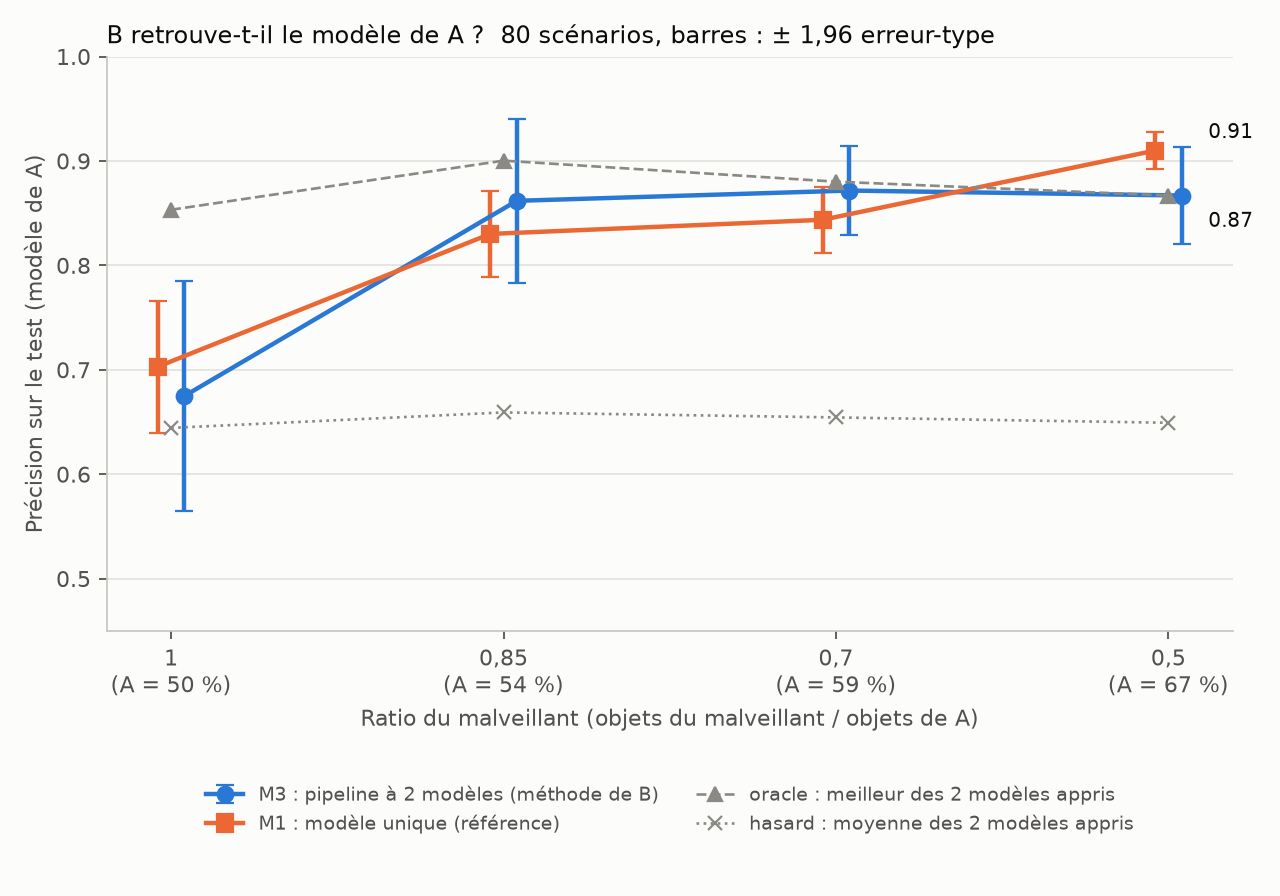
\includegraphics[width=\textwidth]{../results/t4_final.png}
\caption{Précision de B selon la quantité envoyée par le malveillant basique. Vingt scénarios par ratio. Les barres valent $\pm 1{,}96$ erreur-type.}
\label{fig:t4}
\end{figure}

\begin{center}
\begin{tabular}{ccccc}
\toprule
Ratio & Modèle unique & Choix de B & Meilleur des deux & Bonne règle \\
\midrule
0,50 & 0,91 & 0,87 & 0,87 & 20/20 \\
0,70 & 0,84 & 0,87 & 0,88 & 19/20 \\
0,85 & 0,83 & 0,86 & 0,90 & 18/20 \\
1,00 & 0,70 & 0,68 & 0,85 & 9/20 \\
\bottomrule
\end{tabular}
\end{center}

Tant que le malveillant envoie moins que A, B désigne la bonne règle dans au moins 18 cas sur 20. Quand il envoie autant, ce choix est bon 9 fois sur 20, soit le niveau d'un pile ou face. La séparation en deux modèles reste bonne : le meilleur des deux atteint encore 0,85. B ne sait plus lequel garder.

Apprendre un seul modèle sur tout le mélange donne une précision du même ordre, pour un temps d'environ 4~s au lieu d'environ 30~s. Des variantes ont été essayées pour rapprocher B du plafond de 0,98 : lui donner le même temps de calcul que le pipeline, retirer les objets mal classés, ou réapprendre sur les objets expliqués par le modèle choisi. Sur 100 scénarios, aucune ne comble l'écart. La figure~\ref{fig:b} le montre. Le plafond, en haut du graphique, est la précision obtenue quand B n'apprend que sur les objets de A.

\begin{figure}[H]
\centering
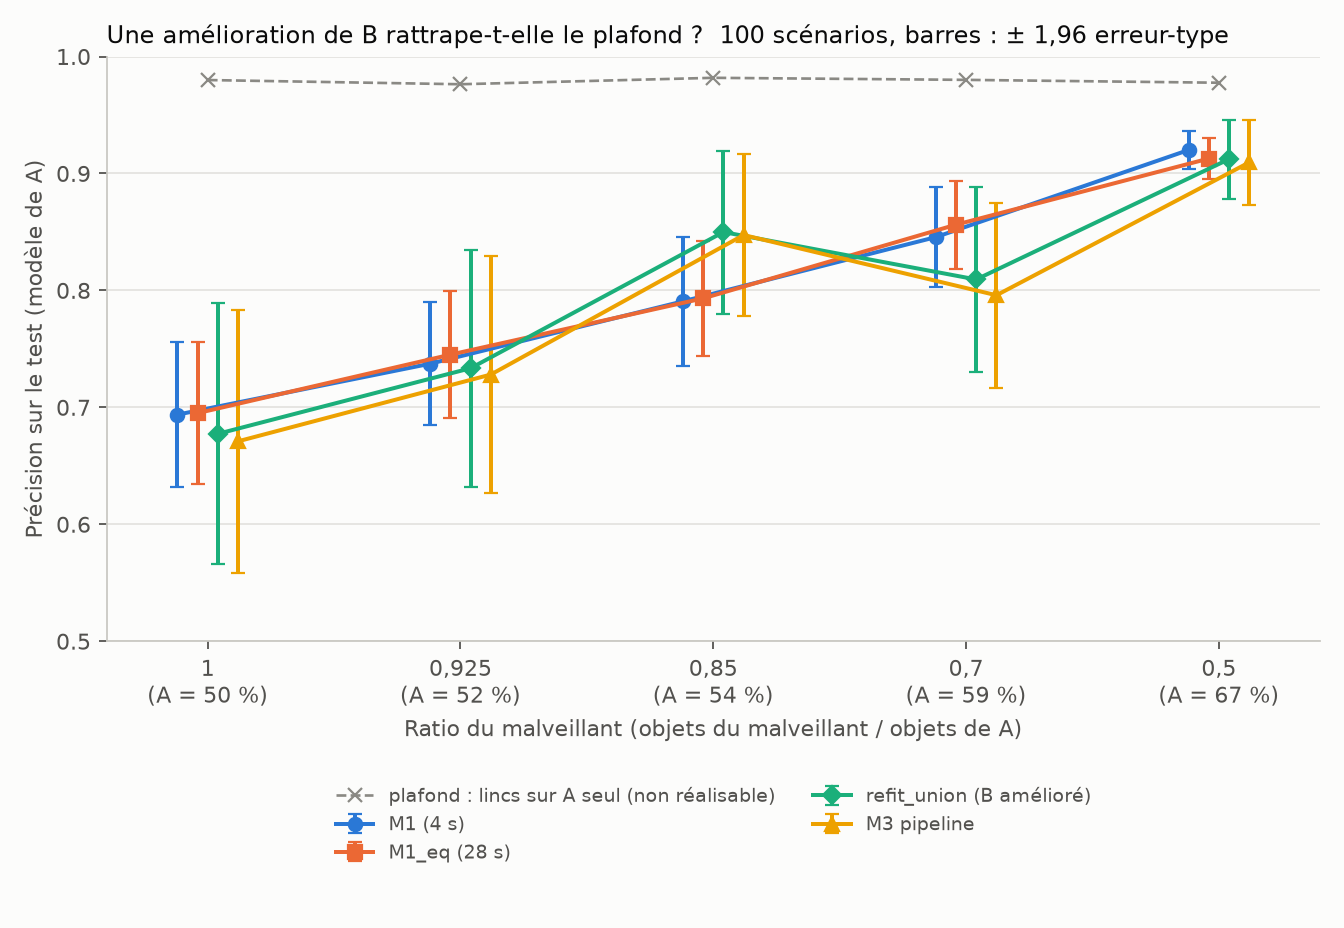
\includegraphics[width=\textwidth]{../results/b_confirm.png}
\caption{Essais pour améliorer B face au malveillant basique. Vingt scénarios par ratio. Le plafond connaît la source de chaque objet ; B ne la connaît pas.}
\label{fig:b}
\end{figure}

\subsection{Autres stratégies de brouillage}

Le malveillant n'a pas accès au modèle de A. Il utilise tout son quota : un objet pour chaque objet de A. Trois stratégies s'ajoutent au tirage au hasard.

\begin{itemize}
\item Modèle extrême. Un seul critère porte le poids, et les seuils sont hauts. Presque tous ses objets tombent dans la catégorie la plus basse.
\item Classe fixe. Chaque objet reçoit la catégorie la plus basse, sans modèle.
\item Deux MR-Sort. Il tire deux modèles et partage ses objets en deux parts égales.
\end{itemize}

La figure~\ref{fig:strat} porte sur 10 scénarios, graines 1100 à 1109. Les objets de A sont les mêmes pour les quatre stratégies d'une graine donnée. Seules les catégories du malveillant changent. Le hasard est le cas où B, après avoir appris deux modèles, en tire un au sort.

\begin{figure}[H]
\centering
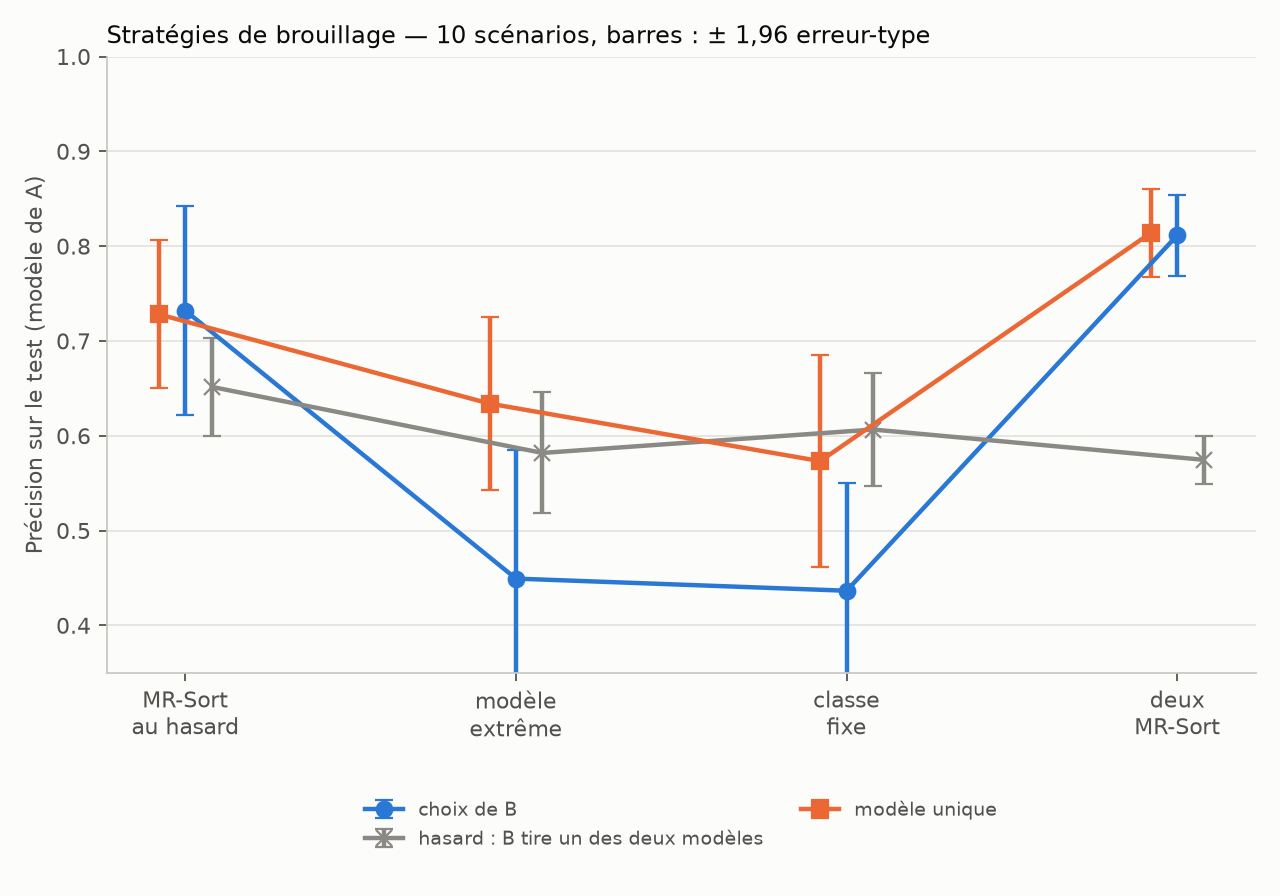
\includegraphics[width=\textwidth]{../results/strategies_multi.png}
\caption{Quatre stratégies, dix scénarios. Les barres valent $\pm 1{,}96$ erreur-type.}
\label{fig:strat}
\end{figure}

\begin{center}
\begin{tabular}{lcccc}
\toprule
Stratégie & Modèle unique & Choix de B & Hasard & Bonne règle \\
\midrule
MR-Sort au hasard & 0,73 & 0,73 & 0,65 & 5/10 \\
Modèle extrême & 0,63 & 0,45 & 0,58 & 2/10 \\
Classe fixe & 0,57 & 0,44 & 0,61 & 2/10 \\
Deux MR-Sort & 0,81 & 0,81 & 0,58 & 10/10 \\
\bottomrule
\end{tabular}
\end{center}

La classe fixe et le modèle extrême gênent B plus que le MR-Sort tiré au hasard. Le choix entre les deux modèles appris devient alors mauvais : B garde la règle du malveillant, et sa précision tombe vers 0,44. Deux MR-Sort gênent peu. Les objets de A restent les plus cohérents, et B retient la bonne règle sur les 10 scénarios.

\section{Conclusion}

Le programme du jalon~1 retrouve un MR-Sort à partir d'exemples classés, avec une précision de test de 0,94 sur la configuration essayée. L'heuristique du jalon~2 trouve deux règles qui expliquent 0,99 des objets sans bruit et 0,91 avec bruit, soit 11 à 12~points de plus que deux modèles appris sur une partition aléatoire. Les proportions des segments ne sont retrouvées qu'approximativement, car une part importante des objets est compatible avec les deux règles. Au jalon~3, cette séparation aide B tant que le malveillant envoie moins d'objets que A. À quota égal, B ne distingue plus les deux règles. Parmi les stratégies qui restent dans le sujet, la plus gênante est d'envoyer des objets tous placés dans la catégorie la plus basse, ou classés par un modèle extrême. B choisit alors souvent la mauvaise règle.

\end{document}
